% !TeX program = xelatex
% !TeX encoding = UTF-8
% !TeX spellcheck = pt_BR
\documentclass[aspectratio=169,10pt]{beamer}
\usepackage[brazilian]{babel}
\usepackage{booktabs}
\usepackage{array}
\usepackage{pgfplots}
\pgfplotsset{compat=1.18}

% Mesmo tema da Etapa 3: claro, sem slides separadores e sem marca-d'água.
\usetheme[nosectionpage,nowatermark]{UEL}
\usetikzlibrary{arrows.meta,calc,positioning}

\setbeamerfont{frametitle}{family=\sffamily,size=\large}
\setbeamerfont{framesubtitle}{family=\sffamily,size=\small}
\setbeamercolor{framesubtitle}{fg=uelgreen}
\newcommand{\chave}[1]{\textcolor{dcblue}{\textbf{#1}}}
\newcommand{\nota}[1]{{\color{dcgreydark}\scriptsize #1\par}}
\newcommand{\numero}[2]{{\color{dcblue}\fontsize{22}{24}\selectfont\textbf{#1}}\par\scriptsize #2}

% Níveis de monitoramento.
\definecolor{nivelok}{HTML}{2E7D32}
\definecolor{nivelatencao}{HTML}{B7791F}
\definecolor{nivelalerta}{HTML}{B3261E}
\newcommand{\ok}{\textcolor{nivelok}{\textbf{OK}}}
\newcommand{\atencao}{\textcolor{nivelatencao}{\textbf{Atenção}}}
\newcommand{\alta}{\textcolor{nivelalerta}{\textbf{Alta}}}
\newcommand{\alerta}{\textcolor{nivelalerta}{\textbf{Alerta}}}

\title[Etapa 4: Governança da solução]{Previsão mensal de internações \\ por doenças crônicas}
\subtitle{Etapa 4 — Governança, monitoramento e entrega final}
\author[André e Vitor]{André Tomonaga Schettini \and Vitor da Costa Garcia}
\institute{Governança de TI e de Dados\\Universidade Estadual de Londrina}
\date{2026}

\begin{document}

\maketitle

% ---------------------------------------------------------------------------
\section{Problema}

\begin{frame}[t]{Problema, objetivos e proposta}
  \vspace{0.05cm}
  \begingroup
  \setbeamercolor{block title}{fg=white,bg=red!75!black}
  \begin{block}{Problema da SESA-PR}
    A demanda por internações de \chave{doenças crônicas} oscila ao longo do ano, gerando
    picos de superlotação e leitos subutilizados.
  \end{block}
  \endgroup

  \vspace{0.25cm}
  \begin{columns}[T,onlytextwidth]
    \begin{column}[T]{0.48\textwidth}
      \begin{block}{Objetivos estratégicos (Etapa 1)}
        \begin{enumerate}
          \item Melhorar a eficiência na \chave{alocação de leitos}
          \item Apoiar \chave{decisões gerenciais} com base em dados
        \end{enumerate}
        \vspace{0.27cm}
      \end{block}
    \end{column}
    \begin{column}[T]{0.48\textwidth}
      \uncover<2->{
        \begin{exampleblock}{Proposta}
          Prever, com \chave{um mês de antecedência}, as AIHs iniciais de quatro grupos DCNT no
          Paraná: circulatórias, diabetes, neoplasias malignas e respiratórias selecionadas.
        \end{exampleblock}
      }
    \end{column}
  \end{columns}

  \vfill
  \uncover<3->{
    \hrule\vspace{0.15cm}
    {\small\textbf{Pergunta da Etapa 4:} depois que o modelo entra em uso, como sabemos de onde ele
    veio, quais são seus riscos e se ele continua funcionando?}
  }
\end{frame}

% ---------------------------------------------------------------------------
\section{Solução}

\begin{frame}{Pipeline e ferramentas}
  \framesubtitle{Sete scripts, cada um com uma saída verificável}
  \centering
  \begin{tikzpicture}[
    etapa/.style={draw=dcgreydark,rounded corners=2pt,minimum width=1.62cm,minimum height=1.15cm,
      align=center,fill=white,font=\sffamily\scriptsize},
    flow/.style={-{Stealth[length=1.6mm,width=1.5mm]},draw=dcgreydark,line width=.8pt},
    saida/.style={font=\sffamily\tiny,text=dcgreydark,align=center,text width=1.7cm},
    stage/.style={line width=2.2pt}
  ]
    \node[etapa] (s1) {\texttt{download}};
    \node[etapa,right=3.2mm of s1] (s2) {\texttt{quality}};
    \node[etapa,right=3.2mm of s2] (s3) {\texttt{preprocessing}};
    \node[etapa,right=3.2mm of s3] (s4) {\texttt{tuning}};
    \node[etapa,right=3.2mm of s4] (s5) {\texttt{evaluation}};
    \node[etapa,right=3.2mm of s5,fill=dcbluetint] (s6) {\texttt{monitoring}};
    \node[etapa,right=3.2mm of s6,fill=dcbluetint] (s7) {\texttt{tracking}};
    \foreach \a/\b in {s1/s2,s2/s3,s3/s4,s4/s5,s5/s6,s6/s7}
      \draw[flow] (\a.east) -- (\b.west);

    \node[saida,below=1.5mm of s1] {212 arquivos\\FTP do DATASUS};
    \node[saida,below=1.5mm of s2] {exclusões\\por motivo};
    \node[saida,below=1.5mm of s3] {768 linhas\\só totais estaduais};
    \node[saida,below=1.5mm of s4] {675 trials\\Optuna};
    \node[saida,below=1.5mm of s5] {teste 2025\\hash da execução};
    \node[saida,below=1.5mm of s6] {completude, drift\\e desempenho};
    \node[saida,below=1.5mm of s7] {experimentos\\e Model Registry};

    \draw[stage,uelgreen] ([yshift=-11mm]s1.south west) -- ([yshift=-11mm]s5.south east)
      node[midway,below=1.2mm,font=\sffamily\small,text=uelgreen]{Entregue na Etapa 3};
    \draw[stage,dcblue] ([yshift=-11mm]s6.south west) -- ([yshift=-11mm]s7.south east)
      node[midway,below=1.2mm,font=\sffamily\small,text=dcblue]{Etapa 4};
  \end{tikzpicture}

  \vfill
  \uncover<2->{
    \footnotesize
    \begin{tabular*}{\linewidth}{@{\extracolsep{\fill}}llll@{}}
      \toprule
      \textbf{Linguagem e dados} & \textbf{Modelagem} & \textbf{Rastreamento} & \textbf{Versionamento} \\
      \midrule
      Python 3.13, pandas, PyArrow & scikit-learn 1.8, Optuna & MLflow 3.17, SQLite & Git, GitHub, SHA-256 \\
      \bottomrule
    \end{tabular*}
  }
\end{frame}

\begin{frame}{Dados e modelo}
  \begin{columns}[T,onlytextwidth]
    \begin{column}[T]{0.50\textwidth}
      \vspace{0pt}
      {\color{uelgreen}\large\textbf{Do registro bruto ao dataset}}\par
      \vspace{0.15cm}
      \footnotesize
      \begin{tabular*}{\linewidth}{@{\extracolsep{\fill}}lr@{}}
        \toprule
        \textbf{SIH/SUS RDPR, 2008-12 a 2026-07} & \textbf{Registros} \\
        \midrule
        Fora do período 2009--2025 & 637.756 \\
        CID J36 (excluído do grupo) & 7.832 \\
        Fora dos quatro grupos DCNT & 10.876.693 \\
        AIHs de continuação & 651 \\
        \chave{AIHs iniciais selecionadas} & \chave{3.608.323} \\
        \midrule
        Total lido & 15.131.255 \\
        \bottomrule
      \end{tabular*}\par
      \vspace{0.12cm}
      \nota{Cada exclusão é contada por arquivo em \texttt{data\_quality.csv}; o script para se os totais não fecharem.}
      \vspace{0.10cm}
      {\small 192 meses $\times$ 4 grupos $=$ \chave{768 linhas} com 13 features do passado e do calendário.}
    \end{column}
    \begin{column}[T]{0.45\textwidth}
      \vspace{0pt}
      \uncover<2->{
        \centering
        {\color{dcblue}\large\textbf{Modelo oficial: MLP 32 $\rightarrow$ 16}}\par
        \vspace{0.15cm}
        \small
        \begin{tabular}{rl}
          Execução & \texttt{20261105T205507} \\
          Ativação e solver & ReLU, L-BFGS \\
          Regularização & $\alpha = 1{,}46$ \\
          Janela de treino & 2010 em diante \\
          Validação 2022--2024 & macro-WAPE 5,28\% \\
          Versão & \texttt{modelo-v1.0.0} \\
        \end{tabular}\par
        \vspace{0.25cm}
        \raggedright
        \nota{Venceu 9 famílias de modelos em 3 janelas de treino, pelo menor erro médio entre os quatro grupos (macro-WAPE).}
      }
    \end{column}
  \end{columns}
\end{frame}

% ---------------------------------------------------------------------------
\section{Governança}

\begin{frame}{Versionamento}
  \framesubtitle{Cada peça tem uma identidade verificável}
  \centering
  \small
  \renewcommand{\arraystretch}{1.25}
  \begin{tabular}{@{}p{2.2cm}>{\raggedright\arraybackslash}p{5.6cm}>{\raggedright\arraybackslash}p{5.2cm}@{}}
    \toprule
    \textbf{Peça} & \textbf{Como é versionada} & \textbf{Como se confere} \\
    \midrule
    Código & Git, branch por marco, PR revisado, merge na \texttt{main} & Tags \texttt{entrega-etapa3} e \texttt{modelo-v1.0.0} \\
    Dados brutos & 212 competências fixas no código & \texttt{preprocessing.py} para se os totais não baterem \\
    Dataset & SHA-256 do arquivo e \chave{do conteúdo} & Totais esperados e hash por execução \\
    Modelo & Pasta imutável por execução; tag \texttt{modelo-v1.0.0}; MLflow & SHA-256 da pasta em \texttt{registry.csv} \\
    Configuração & \texttt{config.json}, \texttt{requirements.txt} com versões exatas & Versões, semente e máquina registradas \\
    \bottomrule
  \end{tabular}

  \vfill
  \uncover<2->{
    \begin{exampleblock}{Versão semântica do modelo}
      \textbf{MAJOR}: muda alvo, features ou modelo \quad
      \textbf{MINOR}: nova busca com dados estendidos \quad
      \textbf{PATCH}: só documentação
    \end{exampleblock}
  }
\end{frame}

\begin{frame}{Rastreabilidade com MLflow}
  \framesubtitle{Do experimento ao modelo em uso}
  \setbeamerfont{block body}{size=\scriptsize}
  \begin{columns}[T,onlytextwidth]
    \begin{column}[T]{0.56\textwidth}
      \vspace{0pt}
      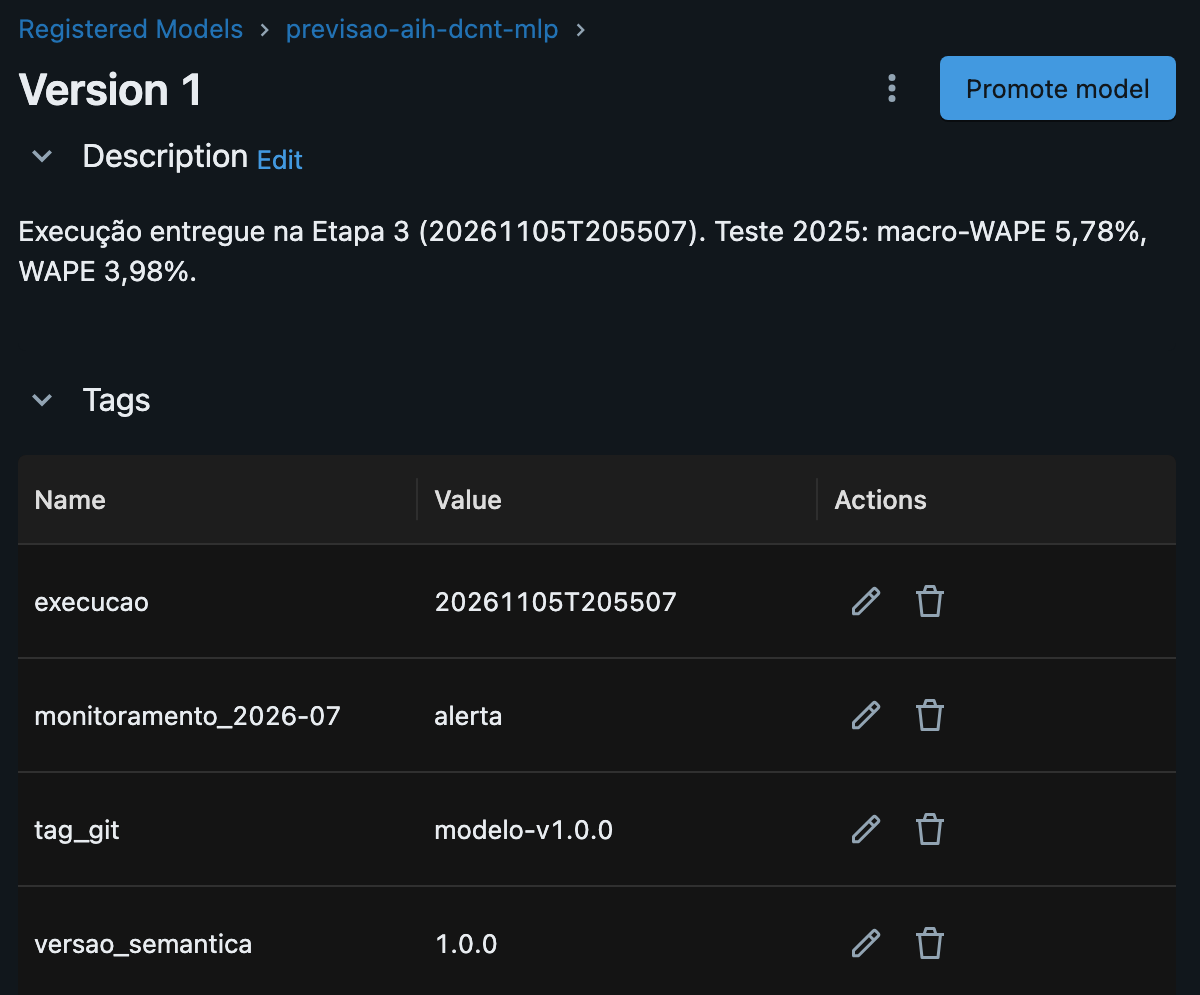
\includegraphics[height=5.3cm]{img/mlflow_registry.png}\par
      \nota{Model Registry: versão 1 (apelido \texttt{champion}), com a execução de origem, a tag Git e o resultado do último monitoramento.}
    \end{column}
    \begin{column}[T]{0.40\textwidth}
      \vspace{0pt}
      \scriptsize
      \begin{block}{O que fica registrado}
        \begin{itemize}
          \item \textbf{Experimento:} execução oficial, reprodução e 54 runs da busca
          \item \textbf{Run:} dados, parâmetros, versões, máquina, métricas e modelo
          \item \textbf{Registry:} versão em uso e por quê
          \item \textbf{Monitoramento:} um run por ciclo, ligado à versão
        \end{itemize}
      \end{block}
      \uncover<2->{
        \begin{alertblock}{Garantias}
          \begin{itemize}
            \item O modelo só é carregado se o hash conferir
            \item O modelo do Registry reproduz as previsões entregues
            \item Promover outra versão é um passo humano
          \end{itemize}
        \end{alertblock}
      }
    \end{column}
  \end{columns}
\end{frame}

\begin{frame}{Documentação}
  \framesubtitle{Model Card e documentação dos dados}
  \begin{columns}[T,onlytextwidth]
    \begin{column}[T]{0.48\textwidth}
      \vspace{0pt}
      \begin{exampleblock}{Usos recomendados}
        \begin{itemize}
          \item Planejamento mensal da demanda estadual
          \item Comparação com a regra do ano anterior
          \item Sempre com revisão humana
        \end{itemize}
      \end{exampleblock}
      \vspace{0.15cm}
      \begin{alertblock}{Usos vedados}
        \begin{itemize}
          \item Decisões sobre pacientes
          \item Corte automático de recursos
          \item Ranquear ou punir hospitais e municípios
        \end{itemize}
      \end{alertblock}
    \end{column}
    \begin{column}[T]{0.48\textwidth}
      \vspace{0pt}
      \uncover<2->{
        {\color{uelgreen}\small\textbf{O que está documentado}}\par
        \vspace{0.12cm}
        \footnotesize
        \begin{itemize}
          \item \textbf{Model Card:} objetivo, dados, métricas por grupo, vieses, limitações, variação entre máquinas
          \item \textbf{Dados:} dicionário das 16 colunas, origem, transformações e qualidade
          \item \textbf{Privacidade:} só três campos dos registros brutos são lidos; só totais estaduais, com no mínimo 470 AIHs por célula, são gravados
          \item \textbf{Cobertura:} o modelo conta internações do SUS, não pessoas nem leitos ocupados
        \end{itemize}
      }
    \end{column}
  \end{columns}
\end{frame}

\begin{frame}{Gestão de riscos}
  \framesubtitle{23 riscos de dados, modelo, privacidade, segurança e ética}
  \centering
  \footnotesize
  \begin{tabular}{@{}lp{5.3cm}cp{5.0cm}@{}}
    \toprule
    \textbf{Risco} & \textbf{Descrição} & \textbf{Nota} & \textbf{Resposta} \\
    \midrule
    D1 & Meses recentes chegam incompletos e parecem queda de demanda & \alta~9 & Corrigir pela curva de completude ou prever mês maduro \\
    M2 & Subestimação sistemática, principalmente em circulatórias & \alta~6 & Viés por grupo monitorado; margem definida pelo planejamento \\
    M6 & O mesmo código gera outro modelo em outra máquina & \alta~6 & Modelo oficial é o arquivo versionado, não um retreino \\
    E1 & Decisão automática de recursos a partir da previsão & \alta~6 & Revisão humana registrada em cada uso \\
    \bottomrule
  \end{tabular}\par
  \vspace{0.10cm}
  \nota{Nota $=$ probabilidade $\times$ impacto, de 1 a 3 cada. Os 19 riscos restantes têm nota de 2 a 4.}

  \vfill
  \uncover<2->{
    \begin{columns}[T,onlytextwidth]
      \begin{column}{0.31\textwidth}\centering\numero{2}{riscos novos, descobertos nesta etapa (D6, M6)}\end{column}
      \begin{column}{0.31\textwidth}\centering\numero{1}{risco confirmado com dados reais (D1)}\end{column}
      \begin{column}{0.31\textwidth}\centering\numero{11}{riscos ligados a indicadores de monitoramento}\end{column}
    \end{columns}
  }
\end{frame}

\begin{frame}{Plano de monitoramento}
  \framesubtitle{19 indicadores, cada um com limite, nível e ação}
  \centering
  \footnotesize
  \begin{tabular}{@{}lcp{4.8cm}p{5.2cm}@{}}
    \toprule
    \textbf{Categoria} & \textbf{Qtd.} & \textbf{Exemplos} & \textbf{Limite e ação} \\
    \midrule
    Dados & 7 & Completude, reconciliação, PSI e KS das razões, extrapolação & Mês com completude abaixo de 95\% fica fora da análise \\
    Modelo & 4 & Macro-WAPE, MLP contra baseline, viés por grupo, erro extremo & Macro-WAPE a partir de 10\% ou viés a partir de 10\%: alerta \\
    Negócio & 4 & Erro evitado, subestimação no trimestre, uso, revisão humana & Decisão sem revisão registrada: incidente \\
    Governança & 4 & Incidentes, reclamações, viés entre grupos, gatilhos de revisão & Hash divergente: interromper o uso \\
    \bottomrule
  \end{tabular}

  \vfill
  \uncover<2->{
    \begin{tikzpicture}[
      box/.style={draw=dcgreydark,rounded corners=2pt,fill=white,align=center,font=\sffamily\scriptsize,minimum height=0.85cm,minimum width=2.1cm},
      flow/.style={-{Stealth[length=1.6mm,width=1.5mm]},draw=dcgreydark,line width=.8pt}]
      \node[box] (a) {DATASUS publica\\nova competência};
      \node[box,right=4mm of a] (b) {\texttt{monitoring.py}};
      \node[box,right=4mm of b] (c) {\ok{} / \atencao{} / \alerta{}};
      \node[box,right=4mm of c] (d) {Revisão humana\\e registro};
      \node[box,right=4mm of d,fill=dcbluetint] (e) {Libera, retém\\ou retreina};
      \foreach \x/\y in {a/b,b/c,c/d,d/e} \draw[flow] (\x) -- (\y);
    \end{tikzpicture}
  }
\end{frame}

% ---------------------------------------------------------------------------
\section{Resultados}

\begin{frame}{Resultados: teste retrospectivo de 2025}
  \framesubtitle{Modelo oficial contra a regra do ano anterior}
  \pgfplotsset{
    barras/.style={
      scale only axis,width=0.62\linewidth,xbar,xmin=0,axis lines*=left,
      axis line style={draw=dcgrey},major tick style={draw=none},xticklabels={},
      ytick=data,y dir=reverse,tick label style={font=\sffamily\scriptsize,text=black},
      nodes near coords,nodes near coords style={font=\sffamily\scriptsize,text=black},
      point meta=x,/pgf/number format/assume math mode=true,/pgf/number format/fixed,
      /pgf/number format/fixed zerofill,/pgf/number format/precision=2,/pgf/number format/use comma,
    }
  }
  \begin{columns}[T,onlytextwidth]
    \begin{column}[T]{0.46\textwidth}
      \vspace{0pt}
      \small
      \begin{tabular*}{\linewidth}{@{\extracolsep{\fill}}lrr@{}}
        \toprule
        \textbf{Métrica} & \textbf{Baseline} & \textbf{MLP} \\
        \midrule
        MAE & 469,81 & \chave{226,22} \\
        RMSE & 626,15 & \chave{332,61} \\
        WAPE & 8,27\% & \chave{3,98\%} \\
        Macro-WAPE & 9,60\% & \chave{5,78\%} \\
        Viés médio & -460,27 & \chave{-146,89} \\
        \bottomrule
      \end{tabular*}\par
      \vspace{0.15cm}
      \nota{\textbf{Baseline:} repete o valor do mesmo mês do ano anterior. Erros em AIHs por mês e grupo.}
    \end{column}
    \begin{column}[T]{0.50\textwidth}
      \vspace{0pt}
      \uncover<2->{
        {\color{uelgreen}\small\textbf{WAPE por grupo em 2025 (\%)}}\par
        \vspace{0.05cm}
        \begin{tikzpicture}
          \begin{axis}[barras,height=3.6cm,xmax=15.5,bar width=8pt,area legend,
            enlarge y limits=0.1167,
            symbolic y coords={Circulatórias,Diabetes,Neoplasias,Respiratórias},
            legend style={at={(1,0.36)},anchor=east,draw=none,fill=none,font=\sffamily\scriptsize}]
            \addplot[fill=dcgrey,draw=none] coordinates {
              (9.49,Circulatórias) (13.05,Diabetes) (3.20,Neoplasias) (12.64,Respiratórias)};
            \addplot[fill=dcblue,draw=none] coordinates {
              (4.13,Circulatórias) (11.62,Diabetes) (2.34,Neoplasias) (5.03,Respiratórias)};
            \legend{Baseline,MLP oficial}
          \end{axis}
        \end{tikzpicture}
      }
    \end{column}
  \end{columns}

  \vfill
  \uncover<3->{
    \hrule\vspace{0.15cm}
    {\small\textbf{Correção em relação à Etapa 3:} os slides mostraram 5,00\%, de um retreino neste
    computador. O modelo entregue e versionado tem \chave{5,78\%}; ele é o oficial.}
  }
\end{frame}

\begin{frame}{Resultados: primeiro ciclo de monitoramento}
  \framesubtitle{Internações de 2026 como dados novos}
  \begin{columns}[T,onlytextwidth]
    \begin{column}[T]{0.50\textwidth}
      \vspace{0pt}
      {\color{uelgreen}\small\textbf{Fração das AIHs já processada}}\par
      \nota{Coortes de 2023--2024, por meses desde a internação}
      \begin{tikzpicture}
        \begin{axis}[
          scale only axis,width=0.80\linewidth,height=3.1cm,
          xmin=-0.3,xmax=4.3,ymin=40,ymax=105,
          xtick={0,1,2,3,4},ytick={50,75,100},
          axis lines*=left,axis line style={draw=dcgrey},
          tick label style={font=\sffamily\scriptsize},
          xlabel={meses depois},xlabel style={font=\sffamily\scriptsize},
          nodes near coords,nodes near coords style={font=\sffamily\scriptsize,above left,inner sep=1pt},
          point meta=y,/pgf/number format/fixed,/pgf/number format/precision=1,
          /pgf/number format/use comma]
          \addplot[draw=nivelalerta,densely dashed,forget plot,nodes near coords={}] coordinates {(-0.3,95) (4.3,95)};
          \node[font=\sffamily\scriptsize,text=nivelalerta,anchor=north east] at (axis cs:4.3,94) {95\%};
          \addplot[dcblue,mark=*,thick] coordinates {(0,50.6) (1,80.4) (2,90.9) (3,99.1) (4,99.9)};
        \end{axis}
      \end{tikzpicture}\par
      \nota{Abaixo de 95\% (linha tracejada), o mês é imaturo: em 2026, maio, junho e julho.}
    \end{column}
    \begin{column}[T]{0.46\textwidth}
      \vspace{0pt}
      \uncover<2->{
        {\color{uelgreen}\small\textbf{Previsão de agosto de 2026}}\par
        \nota{Usando os dados como chegam, contra a correção pela curva}
        \vspace{0.10cm}
        \footnotesize
        \begin{tabular*}{\linewidth}{@{\extracolsep{\fill}}lrrr@{}}
          \toprule
          \textbf{Grupo} & \textbf{Sem} & \textbf{Com} & \textbf{Dif.} \\
          \midrule
          Circulatórias & 8.068 & 11.069 & -27\% \\
          Diabetes & 460 & 575 & -20\% \\
          Neoplasias & 4.735 & 7.363 & -36\% \\
          Respiratórias & 3.743 & 5.708 & -34\% \\
          \bottomrule
        \end{tabular*}\par
        \vspace{0.15cm}
        {\small Sem correção, a previsão sai \chave{20\% a 36\% menor}: o atraso parece queda de demanda.}
      }
    \end{column}
  \end{columns}

  \vfill
  \uncover<3->{
    \nota{\textbf{Integridade:} as 768 combinações de 2010--2025, recalculadas com o lote novo, são idênticas ao dataset oficial. Nenhuma célula zerada nem feature ausente em 2026.}
  }
\end{frame}

\begin{frame}{Resultados: desempenho em 2026}
  \framesubtitle{Janeiro a abril, os quatro meses maduros}
  \begin{columns}[T,onlytextwidth]
    \begin{column}[T]{0.52\textwidth}
      \vspace{0pt}
      \footnotesize
      \begin{tabular*}{\linewidth}{@{\extracolsep{\fill}}lrrl@{}}
        \toprule
        \textbf{Indicador} & \textbf{MLP} & \textbf{Baseline} & \textbf{Nível} \\
        \midrule
        WAPE total & 5,62\% & 6,08\% & \ok \\
        Macro-WAPE & 6,72\% & 6,32\% & \alerta \\
        Viés em diabetes & -9,86\% & +1,07\% & \atencao \\
        Viés em circulatórias & -2,36\% & -4,69\% & \ok \\
        \bottomrule
      \end{tabular*}\par
      \vspace{0.12cm}
      \nota{O alerta de macro-WAPE é a MLP perdendo para o baseline, não o erro passando de 7,5\%.}
      \vspace{0.15cm}
      {\color{uelgreen}\small\textbf{Drift}}\par
      \footnotesize
      \begin{itemize}
        \item 2026 cresceu menos que 2023--2025 (razão sazonal: \alerta)
        \item Circulatórias 11,6\% acima do maior valor visto no treino
      \end{itemize}
    \end{column}
    \begin{column}[T]{0.44\textwidth}
      \vspace{0pt}
      \uncover<2->{
        \begin{block}{Decisão registrada}
          \footnotesize
          \begin{itemize}
            \item Não usar maio a julho sem correção
            \item \textbf{Não retreinar ainda:} só 4 meses maduros, e a diferença cabe na variação numérica do modelo
            \item Preparar a versão 1.1.0, com 2025 no treino
            \item Avisar o planejamento sobre a subestimação em diabetes
          \end{itemize}
        \end{block}
      }
      \uncover<3->{
        \vspace{0.10cm}
        \nota{\textbf{Teste dos indicadores:} um surto simulado em respiratórias e uma falha de carga em diabetes acionaram os indicadores esperados.}
      }
    \end{column}
  \end{columns}
\end{frame}

% ---------------------------------------------------------------------------
\section{Desafios}

\begin{frame}{Desafios}
  \setbeamerfont{block body}{size=\scriptsize}
  \begin{columns}[T,onlytextwidth]
    \begin{column}[T]{0.48\textwidth}
      \vspace{0pt}
      \begin{block}{Pipeline simplificada}
        A Etapa 3 trocou um pipeline extenso por sete scripts. A governança da Etapa 4 foi refeita sobre a versão entregue.
      \end{block}
      \vspace{0.08cm}
      \begin{block}{Mesmos dados, outro modelo}
        Mesmo código, dados e bibliotecas geram outra MLP no Debian/Ryzen e no macOS/M4. Uma diferença de $10^{-16}$ numa feature move o macro-WAPE de 5,35\% a 5,72\%.
      \end{block}
      \vspace{0.08cm}
      \begin{block}{Hash de bytes contra hash de conteúdo}
        O mesmo dataset tem outro SHA-256 em outra máquina e bloqueava a avaliação. Passamos a comparar também o conteúdo.
      \end{block}
    \end{column}
    \begin{column}[T]{0.48\textwidth}
      \vspace{0pt}
      \begin{block}{Atraso de processamento}
        Metade das AIHs chega no mês da internação. O teste de 2025, com séries consolidadas, não mostrava esse risco.
      \end{block}
      \vspace{0.08cm}
      \begin{block}{Pandemia}
        Em 2020 o erro da MLP subiu de 4,13\% para 10,62\%. Uma ruptura assim só é tratável com monitoramento e revisão humana.
      \end{block}
      \vspace{0.08cm}
      \begin{block}{Ferramentas}
        O MLflow completo rebaixaria o PyArrow fixado na entrega. Usamos o \texttt{mlflow-skinny} em requisitos separados.
      \end{block}
    \end{column}
  \end{columns}
\end{frame}

% ---------------------------------------------------------------------------
\section{Conclusão}

\begin{frame}{Atendimento aos objetivos estratégicos}
  \centering
  \footnotesize
  \begin{tabular}{@{}p{3.2cm}p{4.6cm}p{5.4cm}@{}}
    \toprule
    \textbf{Objetivo} & \textbf{O que a solução entrega} & \textbf{O que falta} \\
    \midrule
    Eficiência na alocação de leitos & Previsão mensal por grupo, com metade do erro da regra do ano anterior & Previsão regional e conversão de internações em leitos ocupados (CNES) \\
    \addlinespace
    Decisões gerenciais com base em dados & Alertas por nível, registro de decisões, Model Card e matriz de riscos & Painel para gestores e uso real da previsão \\
    \bottomrule
  \end{tabular}

  \vfill
  \begin{columns}[T,onlytextwidth]
    \begin{column}{0.48\textwidth}
      \centering\numero{Parcial}{nos dois objetivos}
    \end{column}
    \begin{column}{0.48\textwidth}
      \centering\numero{7 de 7}{produtos de governança entregues}
    \end{column}
  \end{columns}

  \vfill
  \nota{\textbf{Prioridade da disciplina:} tornar o modelo governável antes de colocá-lo num painel. Um painel sobre um modelo sem monitoramento ampliaria o risco de uso indevido.}
\end{frame}

\begin{frame}{Limitações, aprendizados e próximos passos}
  \begin{columns}[T,onlytextwidth]
    \begin{column}[T]{0.31\textwidth}
      \vspace{0pt}
      {\color{nivelalerta}\small\textbf{Limitações}}\par
      \vspace{0.10cm}
      \scriptsize
      \begin{itemize}
        \item Previsão estadual, em internações, não em leitos
        \item Só 4 meses maduros para avaliar 2026
        \item Curva de completude única para os grupos
        \item Indicadores de negócio ainda não exercidos
      \end{itemize}
    \end{column}
    \begin{column}[T]{0.31\textwidth}
      \vspace{0pt}
      {\color{uelgreen}\small\textbf{Aprendizados}}\par
      \vspace{0.10cm}
      \scriptsize
      \begin{itemize}
        \item \textbf{Versionar o artefato}, não só o código: retreinar não reproduz o modelo
        \item O \textbf{monitoramento} revelou riscos que o teste retrospectivo escondia
        \item Registrar a \textbf{máquina} faz parte da rastreabilidade
        \item Corrigir um número publicado também é governança
      \end{itemize}
    \end{column}
    \begin{column}[T]{0.31\textwidth}
      \vspace{0pt}
      {\color{dcblue}\small\textbf{Próximos passos}}\par
      \vspace{0.10cm}
      \scriptsize
      \begin{enumerate}
        \item Corrigir os meses incompletos
        \item Retreinar com 2025 (v1.1.0)
        \item Mais três ciclos de monitoramento
        \item Regiões de saúde, com avaliação de privacidade
        \item Leitos (CNES) e painel para gestores
      \end{enumerate}
    \end{column}
  \end{columns}

  \vfill
  \hrule\vspace{0.15cm}
  {\small\textbf{Recomendação:} usar a previsão como apoio ao planejamento, com revisão humana, depois de corrigir os meses incompletos.}
\end{frame}

\obrigado[Perguntas?]

% ---------------------------------------------------------------------------
% Slides de apoio: fora da numeração principal.
\begin{frame}[plain,noframenumbering]{Apoio: por que o modelo muda entre máquinas}
  \begin{columns}[T,onlytextwidth]
    \begin{column}[T]{0.55\textwidth}
      \vspace{0pt}
      \footnotesize
      \begin{tabular*}{\linewidth}{@{\extracolsep{\fill}}llrr@{}}
        \toprule
        \textbf{Execução} & \textbf{$\alpha$} & \textbf{WAPE} & \textbf{Macro} \\
        \midrule
        Entregue (oficial) & 1,46 & 3,98\% & 5,78\% \\
        Retreino da entregue neste Mac & 1,46 & 4,15\% & 5,72\% \\
        Busca refeita neste Mac & 0,71 & 3,70\% & 5,00\% \\
        \bottomrule
      \end{tabular*}\par
      \vspace{0.25cm}
      \begin{tabular*}{\linewidth}{@{\extracolsep{\fill}}lr@{}}
        \toprule
        \textbf{Treino com $\alpha = 1{,}46$} & \textbf{Macro-WAPE} \\
        \midrule
        Dados originais & 5,72\% \\
        \texttt{mes\_seno} $+$ 1 ulp ($\approx 10^{-16}$) & 5,35\% \\
        \texttt{media\_movel\_3} $+$ 1 ulp & 5,56\% \\
        \bottomrule
      \end{tabular*}
    \end{column}
    \begin{column}[T]{0.40\textwidth}
      \vspace{0pt}
      \footnotesize
      \begin{itemize}
        \item O Optuna sorteia valores que diferem na 16ª casa entre máquinas
        \item A MLP com L-BFGS amplifica essa diferença
        \item A busca refeita aqui coincide em 664 de 675 trials com a do pipeline antigo
        \item O conteúdo do dataset é idêntico nas três máquinas; só os bytes do arquivo mudam
      \end{itemize}
      \vspace{0.15cm}
      \begin{exampleblock}{Consequência}
        O modelo oficial é o arquivo versionado. Retreino e comparação de versões sempre na mesma máquina.
      \end{exampleblock}
    \end{column}
  \end{columns}
\end{frame}

\begin{frame}[plain,noframenumbering]{Apoio: o pacote de entrega}
  \centering
  \footnotesize
  \begin{tabular}{@{}l>{\raggedright\arraybackslash}p{9.6cm}@{}}
    \toprule
    \textbf{Exigência} & \textbf{Onde está no repositório} \\
    \midrule
    1. Repositório & \texttt{solucao/} com os scripts e \texttt{requirements.txt}; \texttt{README.md} com a reprodução \\
    2. Dataset documentado & \texttt{entrega-etapa4/dataset-documentado.md}, \texttt{solucao/results/data\_quality.csv} \\
    3. Registro dos experimentos & \texttt{entrega-etapa4/registro-experimentos.md}, \texttt{solucao/results/} \\
    4. Model Card & \texttt{entrega-etapa4/model-card.md} \\
    5. Plano de monitoramento & \texttt{entrega-etapa4/plano-monitoramento.md} \\
    6. Matriz de riscos & \texttt{entrega-etapa4/matriz-riscos.md} \\
    7. Relatório executivo & \texttt{entrega-etapa4/relatorio-executivo.md} \\
    \bottomrule
  \end{tabular}

  \vfill
  \nota{A documentação técnica detalhada fica em \texttt{solucao/docs/}. Todos os números dos slides vêm de \texttt{solucao/results/}.}
\end{frame}

\end{document}
